\justifying
\NSFCBodyText

\subsubsection{研究背景}

机器人被誉为“制造业皇冠顶端的明珠”，是实现高端制造自主可控、构建现代化产业体系的核心装备\upcite{robot2021}。
在“十五五”规划的指引下，以具身智能机器人为代表的新一代机器人技术，被定位为推动新质生产力发展的关键未来产业，其智能化与自主化水平的提升，将为实现产业升级提供坚实支撑\upcite{policy2025}。
然而，当前机器人广泛采用插拔式有线充电方式，其物理连接的固有限制以及繁琐的人工介入，已成为制约其向高级别自主运行演进、充分释放其作为新质生产力效能的“卡脖子”难题。%突出瓶颈
\textbf{磁耦合式无线电能传输（Inductive Power Transfer, IPT）技术}利用线圈之间的耦合磁场能在一定的间距内实现能量的非接触传输，被列为“十项引领未来的科学技术”之一\upcite{kurs2007wireless,covic2013inductive}。

\begin{figure}[!h]
	\centering
	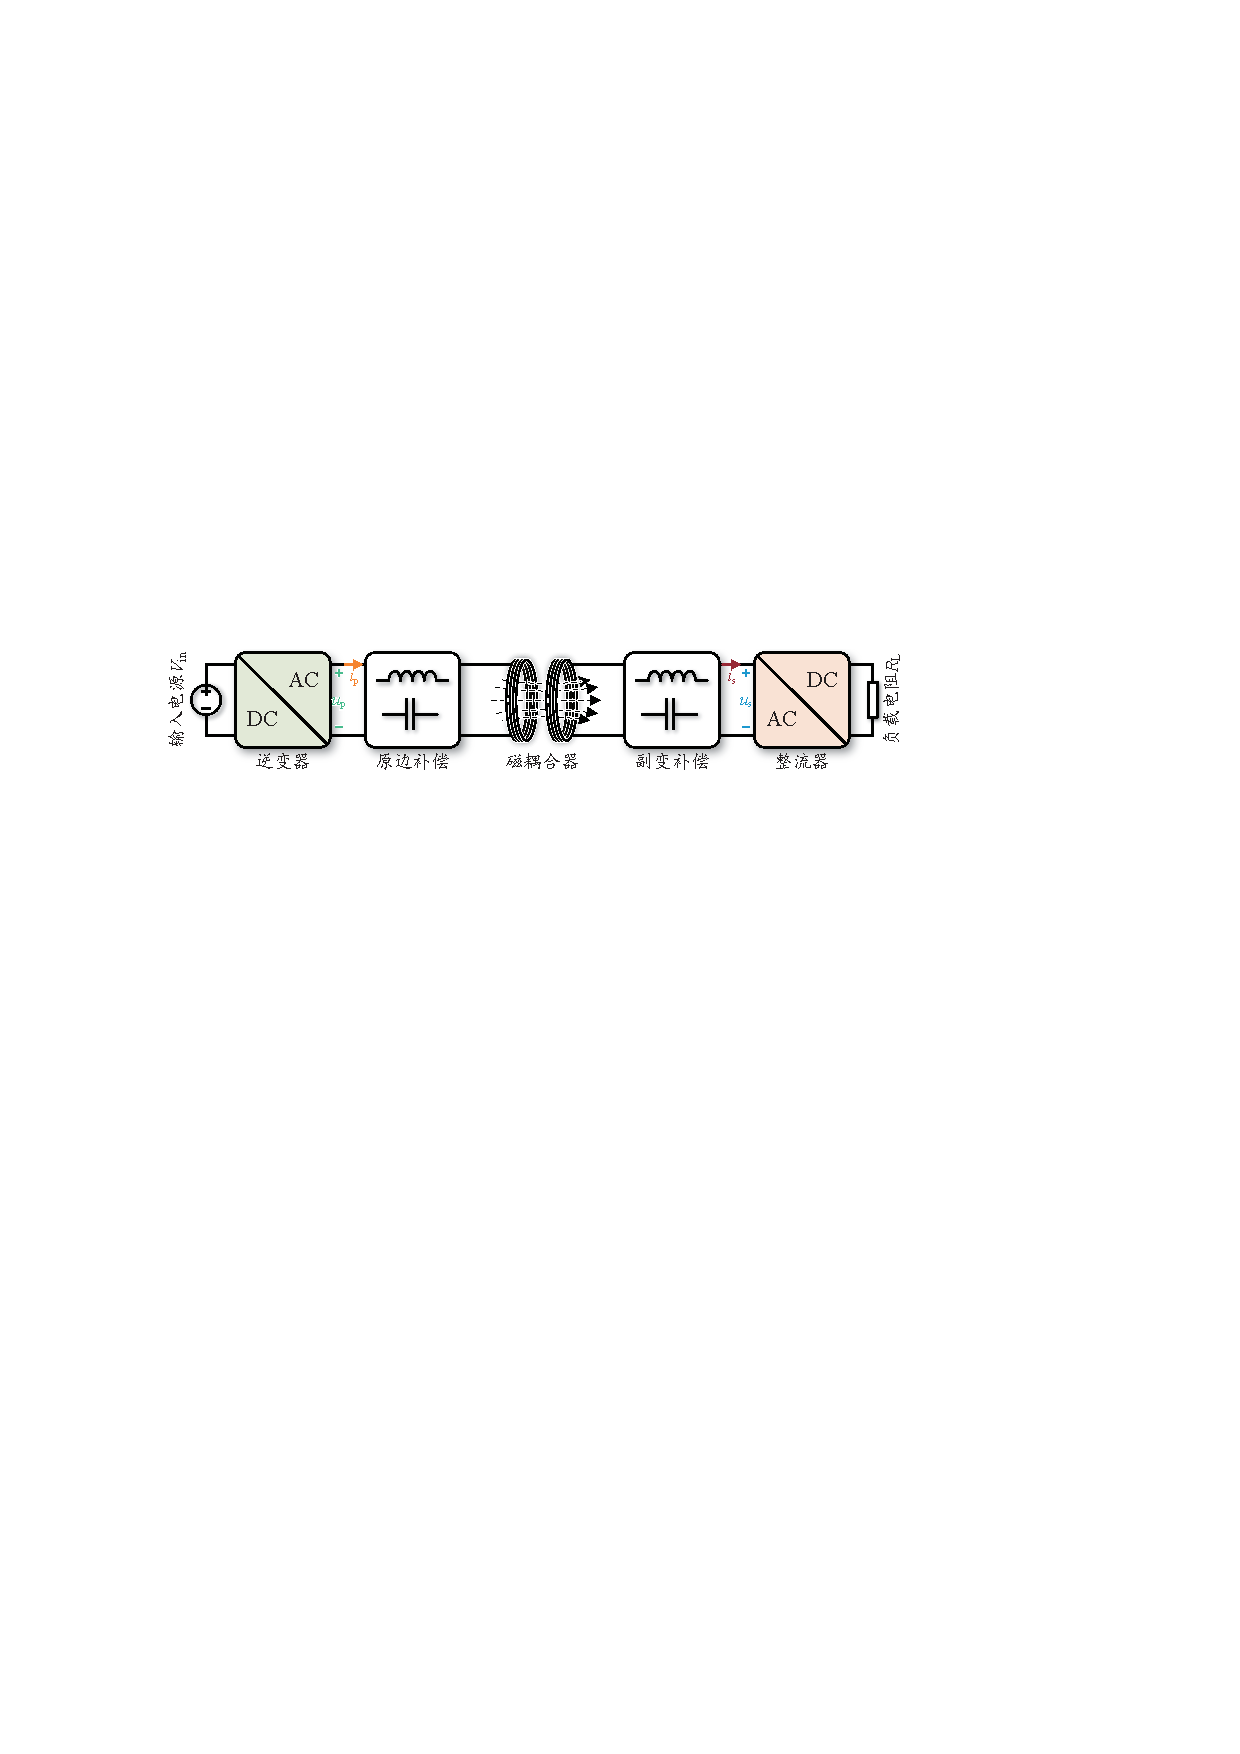
\includegraphics[width=13.5cm]{./figures/IPT_system_framework.pdf}
	\caption{无线快充\dots} 
	\label{fig:strong_IPT_application}
\end{figure}


综上，\dots

\subsubsection{国内外研究现状}

由上述的介绍可知，\dots

\textbf{因此，\dots}


\subsubsection{研究思路}

\textbf{据此，\dots}。
